% Screening Tasks for Agentic Automation -- companion to design_process.tex, hand-maintained.
% Evidence base: 22 papers in ../articles/ and ../articles/batch3/ (read October 2026).
\documentclass[10pt]{article}
\usepackage[T1]{fontenc}
\usepackage[utf8]{inputenc}
\usepackage{lmodern}
\usepackage[letterpaper,margin=2.2cm]{geometry}
\usepackage{microtype}
\usepackage{xcolor}
\usepackage{array,booktabs,tabularx,longtable}
\usepackage{enumitem}
\usepackage{amssymb}
\usepackage{parskip}
\usepackage[most]{tcolorbox}
\usepackage[colorlinks=true,linkcolor=blue!55!black,urlcolor=teal!55!black,citecolor=blue!55!black]{hyperref}
\usepackage{tikz}
\usetikzlibrary{arrows.meta,backgrounds,calc,positioning}

\setlist{itemsep=1pt,topsep=2pt}
\setlength{\LTcapwidth}{\linewidth}
\newcolumntype{L}{>{\raggedright\arraybackslash}X}
\newcolumntype{P}[1]{>{\raggedright\arraybackslash}p{#1}}

% Diagram style shared with design_process.tex
\definecolor{dpbg}{HTML}{F3F4F6}
\definecolor{dpline}{HTML}{C3C8CF}
\definecolor{dpink}{HTML}{2B2F36}
\definecolor{dpmute}{HTML}{6B7280}
\definecolor{dpcoral}{HTML}{E2683C}
\definecolor{dpcoralbg}{HTML}{FBE4DA}
\newcommand{\dpmono}{\fontfamily{zi4}\selectfont}
\tikzset{
  dp/.style={font=\sffamily\scriptsize, color=dpink, >={Stealth[length=4pt,width=3.5pt]},
    show background rectangle, inner frame xsep=10pt, inner frame ysep=8pt,
    background rectangle/.style={fill=dpbg, draw=none}},
  box/.style={draw=dpline, fill=white, line width=0.5pt, rounded corners=1.5pt, align=center, inner sep=5pt, minimum height=1.05cm},
  focal/.style={box, draw=dpcoral, fill=dpcoralbg},
  flow/.style={->, draw=dpink, line width=0.6pt},
  back/.style={->, draw=dpmute, dashed, line width=0.6pt},
  lab/.style={font=\dpmono\tiny, text=dpmute, inner sep=1.5pt},
}

\newtcolorbox{goal}{colback=blue!4,colframe=blue!45!black,boxrule=0.5pt,arc=1pt,left=4pt,right=4pt,top=2pt,bottom=2pt}
\newtcolorbox{gate}{colback=green!5,colframe=green!40!black,boxrule=0.5pt,arc=1pt,left=4pt,right=4pt,top=2pt,bottom=2pt,title=Done when,fonttitle=\sffamily\bfseries\small}
\newtcolorbox{example}[1]{colback=black!3,colframe=black!35,boxrule=0.4pt,arc=1pt,left=4pt,right=4pt,top=2pt,bottom=2pt,title={Example: #1},fonttitle=\sffamily\bfseries\small,fontupper=\small}
\newcommand{\inferred}{\textsf{\small[inferred]}}
\newcommand{\p}[1]{\textsuperscript{[#1]}}

\title{\textbf{Screening Tasks for Agentic Automation}\\[4pt]
\large A companion to the Agentic System Design Process: what to check between Phase~1 and Phase~2}
\author{J. A. Arroyo}
\date{Version 0.9 --- 10 October 2026}

\begin{document}
\maketitle

\begin{abstract}
\noindent This document gives a first screen for deciding, before building anything, whether a task is worth testing with a language model and, separately, whether to test an agent.
The explanation is short: look for an expert who spends their time carrying results between tools that already work, where there is evidence to judge the result against; then ask whether a fixed procedure, with its branches and retries, can do the job.
Each point is illustrated with systems from 22 selected papers and preprints, listed in the appendix: nine from one engineering and materials-science group and thirteen from other groups.
\textbf{The screen is my inference from recurring cases in those papers. None of them tests it as a predictive rule.}
\inferred{} marks a statement the papers do not themselves make.
\end{abstract}

\begin{tcolorbox}[colback=black!3,colframe=black!35,boxrule=0.4pt,arc=1pt,left=4pt,right=4pt,top=2pt,bottom=2pt,title={One set of three documents},fonttitle=\sffamily\bfseries\small]
\small
\begin{enumerate}[leftmargin=1.4em,itemsep=0pt]
\item \textbf{Learning to Build Agentic Systems} (the guide): the courses, lectures and assignments behind the practices. \emph{Use it to learn a topic.}
\item \textbf{Agentic System Design Process}: nine phases from framing a problem to running it in production. \emph{Use it to design a system.}
\item \textbf{Screening Tasks for Agentic Automation}: a one-page worksheet, filled in after Phase~1 of the design process, that feeds Phase~2 and sets up the comparison run in Phase~7. \emph{Use it to decide whether a task is worth it.}
\end{enumerate}
This is document~3. Phase numbers and the four options (deterministic code, single LLM call, fixed workflow, bounded agent) are those of the design process\p{D}; the courses behind it are indexed in the guide\p{G}.
\end{tcolorbox}

\section{The idea}

Much expert work with software has the same shape.
The expert runs a tool, reads what came out, decides what to try next, prepares the input for the next tool, and repeats until a check says the result is good enough.
The tools do the computing.
The person is the connection between them (Figure~\ref{fig:glue}).

\begin{figure}[htbp]
\centering
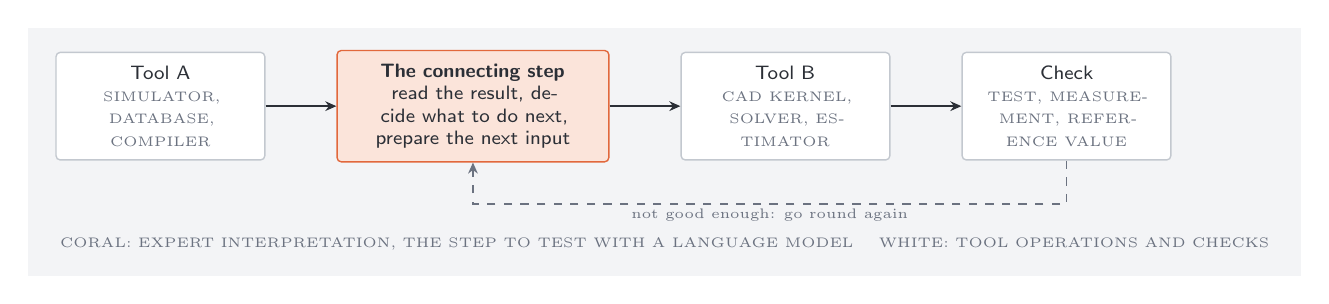
\begin{tikzpicture}[dp, node distance=0.9cm]
\node[box, text width=2.3cm] (a) {Tool A\\{\dpmono\tiny\color{dpmute}SIMULATOR, DATABASE, COMPILER}};
\node[focal, text width=3.1cm, right=of a] (g) {\textbf{The connecting step}\\read the result, decide what to do next, prepare the next input};
\node[box, text width=2.3cm, right=of g] (b) {Tool B\\{\dpmono\tiny\color{dpmute}CAD KERNEL, SOLVER, ESTIMATOR}};
\node[box, text width=2.3cm, right=of b] (c) {Check\\{\dpmono\tiny\color{dpmute}TEST, MEASUREMENT, REFERENCE VALUE}};
\draw[flow] (a) -- (g);
\draw[flow] (g) -- (b);
\draw[flow] (b) -- (c);
\draw[back] (c.south) -- ++(0,-0.55) -| node[lab, pos=0.25, below] {not good enough: go round again} (g.south);
\node[lab, anchor=west] at ([yshift=-1.75cm]a.west) {CORAL: EXPERT INTERPRETATION, THE STEP TO TEST WITH A LANGUAGE MODEL \quad WHITE: TOOL OPERATIONS AND CHECKS};
\end{tikzpicture}
\caption{A recurring pattern: expert interpretation connects tool operations and checks. The tools must be usable and the checks tested; some checks stay with a person. The arrangement is my synthesis \inferred.}
\label{fig:glue}
\end{figure}

The connecting step is worth testing with a language model when three things are true:
\begin{enumerate}
\item \textbf{There is a connecting step.} Someone has to interpret a result before the next tool can run, and that interpretation is hard to write as rules.
\item \textbf{The tools can run.} Software does the calculating and simulating. The model may still have to form hypotheses, choose assumptions and interpret results, and those judgments need checking too.
\item \textbf{Something checks the result.} A test, a measurement, a reference value or a calibrated expert review says whether a step worked.
\end{enumerate}

That is the whole of the first question. Passing it justifies a trial, not a prediction of success, and it says nothing yet about agents.
The second, separate question is: \textbf{can a fixed procedure, with its branches and retries, do the job?}
If it can, the system is a fixed workflow, the model fills in the connecting step at set points, and that is what to test first.
If important decisions are left unresolved, compare it with a version in which the model chooses the next action from the results and decides when to stop or escalate.
That component is an agent, and whether it earns its extra cost is something to test, not assume.

\begin{example}{a rocket, and a software bug}
\textbf{RocketSmith}\p{2} designs high-powered rockets. A flight simulator, a CAD kernel and a slicer already exist; an engineer normally iterates between them, updating mass estimates and checking that the design still meets its stability target. The paper names its motivation as ``friction between the various software tools'' and notes that ``delegating these numerically precise tasks to tools would result in accurate responses''\p{2, pp.\,2,\,6}. The connecting step is the engineer; the checks are simulated stability, slicer mass and, in the end, four flights.

\textbf{TDFlow}\p{8} repairs software defects. The tools are the repository and its tests; the connecting step is reading the code and writing a patch; the check is whether the tests pass. Its order of steps is written in advance: the system ``prevents the LLM from deciding future actions''\p{8, p.\,3}. The outer procedure is fixed, with small tool-using agents inside its stages. Given human-written tests, it reports 88.8\% success on 278 attempted SWE-bench Lite cases\p{8, pp.\,5,\,11}.
\end{example}

The two examples have the same shape, and both mix a fixed procedure with parts where the model chooses. TDFlow states its fixed outer workflow outright; RocketSmith also prescribes a sequence of skills\p{2, p.\,19}. So ask the second question about one component at a time.
The rest of this document turns each question into things you can check from existing work.

\paragraph{What this replaces.}
A natural first guess is that the good opportunities are tasks where rules written in code hit a hard wall.
The papers do not establish that as a way to choose an agent.
In the systems I read, software usually does the calculation, the simulation and the check, and a model does the interpreting, generating or coordinating.
That is how the authors divided the work. It does not show that rules or conventional methods could not do the model's share.
And a limit of rules does not by itself call for an agent, because a single model call and a fixed workflow get past rules too.

\section{Scope: jobs that end, and services that keep watch}\label{sec:scope}

Before screening a task, say how the system would run. There are two cases \inferred:
\begin{itemize}
\item \textbf{On demand.} A person or another program hands the system a piece of work. It runs, and it ends when that work ends.
\item \textbf{Always on.} The system stays responsible for \emph{noticing} that work is needed as events arrive, and may start a bounded run when one does.
\end{itemize}

This is an engineering distinction that I define here; I found no source that establishes it as a taxonomy.
The closest is Lu et al.\p{25}, who contrast agents that need an explicit instruction with an agent that predicts a useful task from observed events. Their agent either proposes help or stays silent, and a proposed task runs only after it is accepted\p{25, \S\S3.1--3.5}.

Four other questions are often folded into this one. They are separate, and each needs its own answer:
\begin{itemize}
\item \emph{How the world behaves.} Whether one decision affects later ones (episodic or sequential) and whether the world changes while the system deliberates (static or dynamic) describe the task environment, not what starts the program. An environment can be both episodic and dynamic\p{23, \S2.3}.
\item \emph{Reacting and taking initiative.} Responding promptly to changes in the environment and taking initiative in pursuit of goals are properties one agent can have together, not two kinds of system. Taking initiative does not require that nobody asked for the goal\p{24, ``A Weak Notion of Agency''}.
\item \emph{Memory.} Keeping information between runs does not mean running without pause. A system can learn across separate jobs\p{26, \S4.1}.
\item \emph{Who approves.} How much the system may decide and do without a person is set on a scale, and separately for gathering information, analysing it, choosing an action and carrying it out\p{27, \S III, Table~I}. An on-demand system can act without approval, and an always-on one can be required to ask.
\end{itemize}
Always on also need not mean that a language model runs all the time. Ordinary code can do the watching and call a model only when something needs interpreting \inferred.

\begin{example}{a monitor that starts a job (an illustration, not from the 22 papers)}
A service watches a stream of readings with fixed thresholds. When a reading drifts out of range, it starts a bounded investigation that gathers evidence, tests explanations and drafts a response. If the response exceeds what the system is authorized to do, it waits for a person. The watching is code; the investigation is a job that ends; the approval rule is a separate decision.
\end{example}

\textbf{What this means for the screen.}
The evaluations reported in the 22 papers concern bounded jobs: a paper, a design brief, a defect or a dataset is handed over and the job ends. None evaluates a service on deciding when a new job should begin \inferred.
That does not settle how every system is deployed; the laser-sintering system also describes process monitoring and overrides during a build\p{5, pp.\,8--12}.
The two questions below are built from those bounded jobs.
For an always-on candidate, screen both the bounded job and the task of noticing when it is needed, starting the second from the simplest option: a threshold, a rule or a conventional model.
This set of papers does not show when the noticing itself benefits from a language model.

\section{First question: is the task worth automating with a language model?}

Start with the simpler answers: could a script, a conventional statistical or machine-learning model, or a numerical optimizer meet the target? Could one model call with the right context do it?
This follows Phase~2 of the design process, which chooses the simplest adequate solution and, checks conventional models and optimizers before the ladder.
If an option meets the target, use it. If you do not know, run the smallest test that would tell you.

\begin{example}{when simple search wins}
\textbf{Pepti-Agent}\p{3} refines peptide sequences against predicted properties. On 24 matched starting sequences that were already feasible, a scripted exhaustive search over single substitutions scored higher than the paper's conservative agent every time, on a score defined by the predictors. Compute and edit depth were not matched, and the manuscript says it ``does not claim'' to outperform simpler search\p{3, pp.\,19,\,22,\,24}.
\end{example}

Then check the three conditions.

\textbf{A1. There is a connecting step.}
Take three to five finished pieces of real work and mark each point where a person had to interpret something before software could proceed: a paper, an error message, a geometric feature, a clinical passage.
Expect most of the surrounding work to be mechanical.

\textbf{A2. The operations can run under your constraints.}
List the operations on each side of the connecting step and how each is reached, including any wrapper, screen interaction or human handoff. Record licence, cost, data access and delay, and which actions the model would be allowed to take. Some physical steps stay with people: RocketSmith leaves fabrication, assembly and flight-readiness work to them, and the laser-sintering study\p{5} leaves handling and physical testing to them alongside its machine-control tools\p{2, pp.\,19--20,\,31; 5, pp.\,11--12}.

\textbf{A3. Something checks the result.}
Name two things, which may differ: the feedback available \emph{while the system runs}, and the \emph{final acceptance check}.
For each, say what kind it is: a \emph{reference} (a test, a measurement, a published value), a \emph{proxy} (a learned predictor), or a \emph{judgment} (a model judge or a human reviewer).
Record what it covers, what it costs, how long it takes and who owns it; try it on a few results you already know to be good and bad; and make sure the final check is something the system cannot alter.
The kind of check limits what the finished system can claim.

\begin{example}{the three conditions in an economics task}
\textbf{Scaling Reproducibility}\p{12} re-runs the replication packages of published studies. \emph{Connecting step:} working out how a package is meant to run and matching its output to the coefficients in the paper's tables. \emph{Tools:} R, Stata and Python already execute the analyses. \emph{Check:} the published coefficients, which are ground truth for reproduction, though not for whether the study's conclusions are right. Of the 254 executable papers, 82\% finished without calling the system's adaptive coordinator. That path still uses model calls to extract metadata and coefficients, so the figure is about adaptive coordination, not all model use\p{12, pp.\,7,\,24}.
\end{example}

\begin{example}{a strong check and a weak one}
The \textbf{Pufibara} benchmark\p{22} tests its private evaluator on known-valid reference models and deliberately off-target submissions. The agent cannot reach that evaluator while revising, or use its verdict for another attempt\p{22, p.\,10}. \textbf{Catalyst-Agent}\p{9} screens catalysts against predicted adsorption energies; when three selected materials were rechecked with a physics calculation, one fell outside the target window\p{9, p.\,32}. Both systems loop successfully, but they support different claims. Agreement is not enough either: in \textbf{GAMESS modernization}\p{18}, matching outputs could share the same build error\p{18, p.\,8}.
\end{example}

\begin{gate}
You can name the connecting step, the operations on either side of it, and a check you have tried on known cases; and you have written down what is known about the simpler options. Passing makes a small model-based baseline worth testing. It does not show that a language model, or an agent, is necessary.
\end{gate}

\section{Second question: does the model need to choose the next step?}

Passing the first question makes a model somewhere in the loop worth trying.
It does not justify an agent.
The published systems give less to go on here: each signal below is drawn from a few cases and has a counterexample in the same set \inferred.

\textbf{B1. Results create decisions that a fixed procedure does not resolve.}
In the same work samples, mark decisions that could not have been made from the original request: looking at a different artifact, asking for a new diagnostic, writing a test, changing approach, stopping, escalating.
Then write the fixed procedure, with its branches, retries and escalation.
If it plausibly covers the workload, build and test it first.
No branch may hide an agent: ``diagnose and repair'' is not a step unless the procedure says how.
Runs that differ from one another, or that retry, are not evidence on their own, because a fixed workflow branches and retries too.

\textbf{B2. An ordinary search or diagnostic routine is not already enough.}
Say what the next decision requires someone to interpret, then compare it with the search, optimization and diagnostic methods available.
``Which parameter value should be tried next?'' is a reason to test an optimizer first. It does not rule a model out, and ``which experiment would explain this failure?'' does not rule one in, since some investigations follow a fixed routine.

\textbf{B3. Handling the exceptions is worth more than it costs.}
Estimate how often the non-routine path occurs, what an expert spends on it, what a miss costs, and what the agent adds in running cost and oversight.
Rare cases with large consequences can matter more than frequent minor ones.

\begin{example}{where choosing the next step shows up}
\textbf{SubDGuide}\p{19} rebuilds a smooth surface from a dense mesh. After a first attempt, its controller may ask for further rendered views before choosing to repair, roll back or stop\p{19, p.\,5}. In \textbf{GAMESS modernization}\p{18}, an agent diagnosing a numerical mismatch wrote its own bisection harness, a step nobody had scripted\p{18, p.\,8}. \textbf{Pufibara}'s agent must ``decide whether to collect further evidence, revise the candidate, or submit it''\p{22, p.\,4}.
\end{example}

\begin{example}{where simpler control remains a credible alternative}
\textbf{Scaling Reproducibility}\p{12} calls its adaptive coordinator when a validation gate fails. Failure patterns that recur are written into deterministic rules or routing branches, through reviewed updates between versions of the pipeline\p{12, pp.\,7,\,9--10}. \textbf{Catalyst-Agent}\p{9} concedes that one of its showcase decisions ``could be interpreted as exhaustive search over a binary parameter''\p{9, p.\,23}. \textbf{SubDGuide}'s refinement stage improves both the output-to-target and the target-to-output P95 distances in 6 of 20 cases and leaves 14 outputs unchanged. It keeps an earlier verified state unless a proposal passes verification and improves the comparison score, which prevents a worse result under that score, not under every measure of quality\p{19, pp.\,5,\,7}. \textbf{TDFlow} reports the simpler Agentless system at \$0.53 per issue and 61.0\% success, against its own \$1.51 and 88.8\%\p{8, pp.\,5,\,11}; the two systems are equipped differently, so this is not a measure of what choosing the next step is worth.
\end{example}

\textbf{B4. Settle it with a matched comparison.}
B1--B3 say where a comparison is worth running.
Only the comparison justifies choosing an agent, and it is the Phase~7 baseline test applied to control:
\begin{itemize}
\item the same model, starting information, tools and check in both arms;
\item comparable limits on calls, time and cost;
\item a fixed workflow that is allowed realistic branches, retries and diagnostic calls (``fixed'' must not mean deprived of feedback);
\item cases that were not used to design either arm.
\end{itemize}
The only difference between the arms is who selects the next step.
None of the 22 papers runs this comparison cleanly (Section~\ref{sec:limits}), which is the main reason the second question cannot be answered from the literature alone.

\begin{gate}
You have written the strongest fixed procedure you can, listed the observed decisions it leaves unresolved, and recorded what evidence would show whether those gaps justify an agent.
\end{gate}

\section{Recap: the whole screen, and where it sits in the design process}\label{sec:recap}

Figure~\ref{fig:recap} puts the pieces in order. The screen starts from the Phase~1 brief of the design process\p{D}, its first three decisions produce the choice that Phase~2 records, and its last step is the comparison that Phase~7 runs.

\begin{figure}[htbp]
\centering
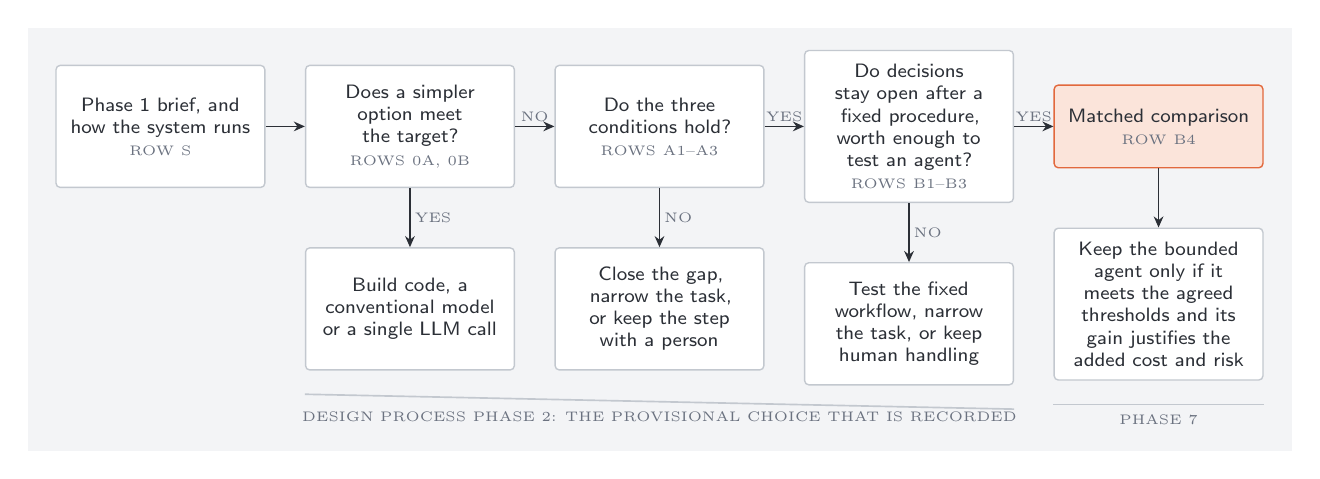
\begin{tikzpicture}[dp, node distance=0.75cm and 0.5cm]
\tikzset{q/.style={box, text width=2.3cm, minimum height=1.55cm}}
\node[q] (q0) {Phase 1 brief, and how the system runs\\{\dpmono\tiny\color{dpmute}ROW S}};
\node[q, right=of q0] (q1) {Does a simpler option meet the target?\\{\dpmono\tiny\color{dpmute}ROWS 0A, 0B}};
\node[q, right=of q1] (q2) {Do the three conditions hold?\\{\dpmono\tiny\color{dpmute}ROWS A1--A3}};
\node[q, right=of q2] (q3) {Do decisions stay open after a fixed procedure, worth enough to test an agent?\\{\dpmono\tiny\color{dpmute}ROWS B1--B3}};
\node[q, focal, right=of q3] (q4) {Matched comparison\\{\dpmono\tiny\color{dpmute}ROW B4}};
\node[q, below=of q1] (o1) {Build code, a conventional model or a single LLM call};
\node[q, below=of q2] (o2) {Close the gap, narrow the task, or keep the step with a person};
\node[q, below=of q3] (o3) {Test the fixed workflow, narrow the task, or keep human handling};
\node[q, below=of q4] (o4) {Keep the bounded agent only if it meets the agreed thresholds and its gain justifies the added cost and risk};
\draw[flow] (q0) -- (q1);
\draw[flow] (q1) -- node[lab, above] {NO} (q2);
\draw[flow] (q2) -- node[lab, above] {YES} (q3);
\draw[flow] (q3) -- node[lab, above] {YES} (q4);
\draw[flow] (q1) -- node[lab, right] {YES} (o1);
\draw[flow] (q2) -- node[lab, right] {NO} (o2);
\draw[flow] (q3) -- node[lab, right] {NO} (o3);
\draw[flow] (q4) -- (o4);
\draw[dpline, line width=0.6pt] ([yshift=-0.3cm]o1.south west) -- ([yshift=-0.3cm]o3.south east)
  node[lab, midway, below=2pt] {DESIGN PROCESS PHASE 2: THE PROVISIONAL CHOICE THAT IS RECORDED};
\draw[dpline, line width=0.6pt] ([yshift=-0.3cm]o4.south west) -- ([yshift=-0.3cm]o4.south east)
  node[lab, midway, below=2pt] {PHASE 7};
\end{tikzpicture}
\caption{The screening decisions and the action each leads to. Row labels refer to the worksheet in Section~\ref{sec:worksheet}. Phase~2 of the design process\p{D} records a provisional choice; a bounded-agent candidate then goes through Phases~3 to~6 before the matched comparison in Phase~7. The lower boxes are actions, not a one-to-one rendering of the four Phase~2 options. Where an answer is unknown, run the cheapest test that would settle it. The arrangement is my synthesis \inferred.}
\label{fig:recap}
\end{figure}

The worksheet's answers are also reused later in the design process, so they are written once:
\begin{center}
\small
\begin{tabularx}{\linewidth}{@{}l L L@{}}
\toprule
Worksheet rows & Design-process phase that uses them & As \\
\midrule
S & Phase 2, scope; Phase 5, design tools, state and context & What starts a job, what notices that work is needed, and what state persists \\
0a, 0b & Phase 2, the alternatives before the ladder and its first two options & Evidence that a simpler option meets or misses the target, or the test needed to decide \\
A1 & Phase 3, decompose and assign ownership & The step the model would own, and the steps that stay with code or a person \\
A2 & Phase 5, design tools, state and context & The tool list, access limits and permitted actions \\
A3 & Phase 4, define the evaluation & The check, its kind, and the known-good and known-bad cases \\
B1--B3 & Phase 2, leaving the fixed workflow & The fixed policy as specified, evidence about what it covers, the decisions it leaves unresolved and their expected value \\
B4 & Phase 7, evaluate, diagnose and iterate & The baseline comparison \\
\bottomrule
\end{tabularx}
\end{center}

\section{Screening worksheet}\label{sec:worksheet}

One page per candidate task. Carry forward the Phase~1 success measure and the limits on cost, delay and failure. Answer from work samples and existing records, and mark each answer as observed, estimated or unknown. Three to five samples are a first look, not a count of how often things happen.

\begin{center}
\small
\begin{tabularx}{\linewidth}{@{}l L L@{}}
\toprule
 & Question & Write down \\
\midrule
S & Does a request start the work, or must the system notice it? (Section~\ref{sec:scope}) & On demand or always on; if always on, the bounded job an event starts, and what does the noticing \\
0a & Would a script, a conventional model or an optimizer meet the target? & The strongest such option; evidence that it meets or misses the target, or ``unknown'' \\
0b & Would one model call with the right context meet it? & Evidence on one call's accuracy and reliability, or the smallest test that would show it \\
A1 & Where does an expert interpret one result to decide the next input? & The step, marked on 3--5 real work samples \\
A2 & Which operations can run under your constraints, and which stay with a person? & Tools and how they are reached; access, cost, delay; human handoffs; permitted actions \\
A3 & What feedback is available during a run, and what is the final check? & For each: reference, proxy or judgment; coverage, cost, delay, owner; outcome on known-good and known-bad cases \\
B1 & Which decisions does the best fixed procedure leave unresolved? & The procedure you wrote, and the decisions it does not cover \\
B2 & Would an ordinary search or diagnostic routine make the next decision? & What the decision requires someone to interpret; the conventional method it was compared with \\
B3 & Is handling the exceptions worth more than it costs? & Frequency from broader records where available; expert time, cost of a miss, added running and oversight cost \\
B4 & What is the best fixed workflow, and how will it be compared? & Both arms, shared limits, untouched test cases \\
\bottomrule
\end{tabularx}
\end{center}

Reading the result \inferred:
\begin{itemize}
\item Evidence supports 0a or 0b: build the simplest option that works and verify it against the Phase~1 success measure.
\item Access or checking is inadequate (A2, A3): close the gap, narrow the task, or leave that step with a person.
\item A fully written fixed procedure plausibly covers the workload: build and test it first. Coverage of the first few samples is provisional.
\item Unresolved decisions remain and are worth enough (B1--B3): compare a bounded agent with the strongest fixed workflow (B4).
\item Where an answer is unknown, write ``unknown'' and run the cheapest check that would settle it.
\end{itemize}

\section{Limits, and where this attaches to the design process}\label{sec:limits}

\textbf{Limits.}
\begin{itemize}
\item \emph{Selection.} The 22 are systems reported in papers and preprints, chosen by me from one group's publication list and from title and abstract searches. They are not a sample of attempted projects and include no failures that went unpublished.
\item \emph{No clean test of the second question.} None of the 22 holds tools, information and budget constant while changing only who selects the next step. SubDGuide comes closest: its rule-based controller shares the evidence and repair tools but also changes initial planning, and its one-shot variant has no feedback stage at all\p{19, pp.\,6--7}. TDFlow compares complete systems with different tools and costs. Gains reported elsewhere could come from better tools, more information, verification or human specification.
\item \emph{Reading depth.} The classifications in the appendix come from text extractions of the methods, evaluation and limitations sections. Figures, code repositories, execution traces and separately hosted supplements were not inspected, and no experiment was rerun.
\item \emph{Not validated.} The screen has not been applied prospectively. Treat a pass as a reason to run the comparison, not as a prediction of its result.
\end{itemize}

\textbf{Attachment to the design process (v1.8)\p{D}.}
Use the worksheet after the Phase~1 gate, as the input to Phase~2; Section~\ref{sec:recap} shows which phase reuses each row.
Three parts of Phase~2 of the design process come from this document:
\begin{enumerate}
\item Before the ladder, a check for alternatives that use no language model (conventional models, optimizers). These are not a rung, since they can also be tools at any rung.
\item Before authorizing a bounded agent, three questions: what observation guides the next decision, what independently checks success, and how that check has been tested.
\item A tighter exit from the fixed-workflow rung. ``Steps cannot be predicted'' is not sufficient, because fixed workflows branch; the strongest maintainable fixed policy and the decisions it leaves unresolved must be written down.
\end{enumerate}

\section*{Authorship and use of AI tools}
\addcontentsline{toc}{section}{Authorship and use of AI tools}

I am the sole author. I used AI tools in preparing this document and disclose their role here.
\begin{itemize}
\item \emph{Claude} (Anthropic, through Claude Code) searched for and read the papers, and drafted and revised the text, the table and the figure under my direction.
\item \emph{Codex} (OpenAI) acted as a second reader. It checked the papers, quotations, numbers and citations, and some sentences follow its suggested corrections closely.
\item The distinction in Section~\ref{sec:scope} started from a conversation I had with \emph{Gemini} (Google). The sources it cited were then checked against the originals.
\end{itemize}
Words taken from a source are in quotation marks with the source and page. Ideas taken from a source are cited to it. Statements marked \inferred{} are my own synthesis.
I set the questions, decided what to include and am responsible for the content.

\appendix
\section{The 22 systems}

Table~\ref{tab:evidence} lists the systems used as examples.
Each reports an applied system in which a language model works with domain tools on an expert's task; papers mainly about evaluation were set aside. This is a purposive selection, not a systematic review.
The last column uses the four options from Phase~2 of the design process: \emph{code}; a \emph{single model call}; a \emph{fixed workflow}, where the path is set in advance, including programmed branches and retries; and an \emph{agent}, where the model chooses the next step from results and decides when it is done.
These assignments are my reading of each paper's methods section, not the authors' label. Several systems fix the outer procedure and keep model-directed components inside it, so a cell describes the level it names and not the whole system.

{\small
\begin{longtable}{@{}r P{3.3cm} P{4.2cm} P{3.9cm} P{3.3cm}@{}}
\caption{The 22 systems: the connecting step automated, what checks the result, and the control structure as built. The control labels and the wording of each cell are mine \inferred.}\label{tab:evidence}\\
\toprule
\# & System & Connecting step & Check & Control as built \\
\midrule
\endfirsthead
\toprule
\# & System & Connecting step & Check & Control as built \\
\midrule
\endhead
\bottomrule
\endfoot
\multicolumn{5}{@{}l}{\emph{One research group (engineering, materials, chemistry)}}\\
1 & Material Database Agent & Reading papers, tables and charts into database rows & Human-built databases, at evaluation only & Four prescribed stages; model-directed delegation and tool-use sessions inside them (agent inside a fixed workflow) \\
2 & RocketSmith & Iterating between flight simulation, CAD and slicer & Simulated stability, slicer mass, four physical flights & Agent tool use inside a prescribed skill sequence; heavy human involvement \\
3 & Pepti-Agent & Choosing the next sequence edit from predictor output & Three learned property classifiers (proxy) & Agent: a single loop with a turn cap \\
4 & AgentsCAD & Choosing a geometry repair for a printing defect & Deterministic overhang recheck and solid validity; a vision-model verifier & Fixed workflow: its agents run ``in a fixed phase order''\p{4, p.\,10} \\
5 & SLS process optimization & Choosing process parameters from past builds & Tensile and flexural tests on printed parts & Agent within a session; people start each build round \\
6 & AgentD & Chaining retrieval, molecule generation and property prediction & Predicted properties and rule filters (proxy) & Fixed workflow in the reported end-to-end run \\
7 & MatSciAgent & Turning a request into database queries or simulations & Tool outputs and repeat-run consistency; little independent validation of correctness & Router plus a per-task model loop (agent) \\
8 & TDFlow & Locating a defect and writing the patch & Reproduction and regression tests & Fixed outer workflow with bounded agents inside \\
9 & Catalyst-Agent & Choosing candidate materials and surface modifications & Predicted adsorption energies (proxy); three DFT checks & Agent at the screening level \\
\midrule
\multicolumn{5}{@{}l}{\emph{Other groups}}\\
10 & Symbolic discovery for fundamental analysis & Proposing valuation equations & Forecast error on held-out quarters & Fixed workflow: a propose--fit--evaluate loop \\
11 & Deploy-Master & Inferring a build environment from documentation & Container build and a minimal run command & Fixed outer pipeline; control inside its refinement step not specified enough to classify \\
12 & Scaling Reproducibility & Running replication packages and matching coefficients & Published coefficients & Fixed outer workflow; an agent diagnoses and repairs on failure \\
13 & HLER & Proposing feasible questions and analyses for a dataset & Two researchers on feasibility; a model reviewer on drafts & Fixed workflow with human gates \\
14 & Causal inference workflow & Turning a causal plan into estimators and diagnostics & Known effects in synthetic benchmarks; diagnostics & Fixed notebook workflow; model-directed control inside it not established \\
15 & Schwartz, Andrews \& Shapiro & Reproducing, speeding up and extending published calculations & Published values, reruns, numerical references; adversarial model judgments for extensions & Fixed outer workflow \\
16 & FinNextAssist & Gathering and reconciling financial evidence & Reference answers; rubric and model-judge grading & Fixed stages with an agent reasoning loop inside \\
17 & CAi Copilot & Choosing molecular generation, filtering and evaluation steps & Rule checks; predicted properties; a blinded model judge & Agent \\
18 & GAMESS modernization & Rewriting legacy Fortran and diagnosing breakage & Compilation, reference outputs, regression tests & Fixed per-file protocol with agent work inside \\
19 & SubDGuide & Planning a control cage, then inspecting and repairing it & Geometric distance to the input mesh; topology gates & Single model call for the plan, then agent refinement \\
20 & Quantum research system & Formalizing a protocol and implementing its calculations & Fixed tests and classical reference calculations & Fixed, approved project graph with agent modules \\
21 & Oncology feature extraction & Mapping clinical documents to a structured schema & Clinician-reviewed values on an annotated subset & Fixed workflow: set routing over code steps and single model calls \\
22 & Pufibara (Modelica) & Deciding what simulation evidence or repair to pursue & Private scenario-based evaluator & Agent \\
\end{longtable}
}

\section*{Sources}
\addcontentsline{toc}{section}{Sources}
Bracketed numbers in the text refer to these entries; page numbers are PDF page positions. arXiv identifiers and DOIs are links.
{\small
\begin{enumerate}[label={[\arabic*]},leftmargin=2.2em]
\item Material Database Agent. \href{https://arxiv.org/abs/2605.04278}{arXiv:2605.04278}.
\item RocketSmith. \href{https://arxiv.org/abs/2606.00097}{arXiv:2606.00097}.
\item Pepti-Agent. \href{https://arxiv.org/abs/2606.15422}{arXiv:2606.15422}.
\item AgentsCAD. \href{https://arxiv.org/abs/2607.02448}{arXiv:2607.02448}.
\item AI agentic selective laser sintering process optimization. \href{https://arxiv.org/abs/2608.25928}{arXiv:2608.25928}.
\item AgentD: LLM agent for modular task execution in drug discovery. \emph{J.\ Chem.\ Inf.\ Model.}\ 66(4), 2026; \href{https://arxiv.org/abs/2507.02925}{arXiv:2507.02925}.
\item MatSciAgent. \emph{Communications Materials} 7, 131 (2026). \href{https://doi.org/10.1038/s43246-025-00994-x}{doi:10.1038/s43246-025-00994-x}.
\item TDFlow: Agentic Workflows for Test Driven Development. EACL 2026; \href{https://arxiv.org/abs/2510.23761}{arXiv:2510.23761}.
\item Catalyst-Agent. \href{https://arxiv.org/abs/2603.01311}{arXiv:2603.01311}.
\item Self-Evolving Multi-Agent Symbolic Discovery for Financial Fundamental Analysis. \href{https://arxiv.org/abs/2609.32746}{arXiv:2609.32746}.
\item Deploy-Master. \href{https://arxiv.org/abs/2601.03513}{arXiv:2601.03513}.
\item Xu and Yang, Scaling Reproducibility: An AI-Assisted Workflow for Large-Scale Replication and Reanalysis. \href{https://arxiv.org/abs/2602.16733}{arXiv:2602.16733}.
\item HLER: Human-in-the-Loop Economic Research via Multi-Agent Pipelines. \href{https://arxiv.org/abs/2603.07444}{arXiv:2603.07444}.
\item A Human-Augmenting Agentic Workflow for Observational Causal Inference. \href{https://arxiv.org/abs/2607.22443}{arXiv:2607.22443}.
\item Schwartz, Andrews and Shapiro, An LLM Workflow That Reproduces, Improves, and Extends Published Economics Research. Working paper, September 2026. \url{https://economics.mit.edu/sites/default/files/2026-09/metascience.pdf}
\item FinNextAssist. \href{https://arxiv.org/abs/2610.03174}{arXiv:2610.03174}.
\item CAi Copilot. \href{https://arxiv.org/abs/2608.06961}{arXiv:2608.06961}.
\item An Agentic Workflow for Legacy HPC Modernization (GAMESS). \href{https://arxiv.org/abs/2608.12249}{arXiv:2608.12249}.
\item SubDGuide. \href{https://arxiv.org/abs/2610.11721}{arXiv:2610.11721}.
\item Demonstration of a Structured Agentic Workflow for Applied Quantum Computing Research. \href{https://arxiv.org/abs/2610.05304}{arXiv:2610.05304}.
\item From Analytics to Tumor Boards: An Evidence-Linked Multi-Agent Workflow for Oncology Feature Extraction. \href{https://arxiv.org/abs/2608.28974}{arXiv:2608.28974}.
\item Pufibara Agent Harness and the Modelica Agent Workflow Benchmark. \href{https://arxiv.org/abs/2608.23653}{arXiv:2608.23653}.
\end{enumerate}
}

\textbf{The other two documents of this set.}
{\small
\begin{enumerate}[leftmargin=2.2em]
\item[{[D]}] J.~A.~Arroyo, \emph{Agentic System Design Process} (v1.8, October 2026). File \texttt{design\_process/design\_process.pdf}.
\item[{[G]}] J.~A.~Arroyo, \emph{Learning to Build Agentic Systems: An instructional compilation guide built from public university courses} (October 2026). File \texttt{guide/agentic\_guide.pdf}.
\end{enumerate}
}

\textbf{Background for Section~\ref{sec:scope}.} These are cited only for the specific points attributed to them there.
{\small
\begin{enumerate}[label={[\arabic*]},leftmargin=2.2em,start=23]
\item S.~Russell and P.~Norvig, \emph{Artificial Intelligence: A Modern Approach}, 4th ed., Pearson, 2020. Chapter~2, \S2.3. \url{https://aima.cs.berkeley.edu/}
\item M.~Wooldridge and N.~R.~Jennings, Intelligent Agents: Theory and Practice. \emph{The Knowledge Engineering Review} 10(2), 115--152, 1995. \href{https://doi.org/10.1017/S0269888900008122}{doi:10.1017/S0269888900008122}.
\item Y.~Lu et al., Proactive Agent: Shifting LLM Agents from Reactive Responses to Active Assistance. ICLR 2025; \href{https://arxiv.org/abs/2410.12361}{arXiv:2410.12361}.
\item T.~R.~Sumers, S.~Yao, K.~Narasimhan and T.~L.~Griffiths, Cognitive Architectures for Language Agents. \emph{Transactions on Machine Learning Research}, 2024; \href{https://arxiv.org/abs/2309.02427}{arXiv:2309.02427}.
\item R.~Parasuraman, T.~B.~Sheridan and C.~D.~Wickens, A Model for Types and Levels of Human Interaction with Automation. \emph{IEEE Transactions on Systems, Man, and Cybernetics, Part A} 30(3), 286--297, 2000. \href{https://doi.org/10.1109/3468.844354}{doi:10.1109/3468.844354}.
\end{enumerate}
}

\end{document}
